\section{Ajuste e interpretação de dados de temperatura}\label{sec:temperatura}

\subsection{Por que esta grandeza?}

A temperatura do ar é uma das grandezas termodinâmicas mais familiares no cotidiano e na experimentação científica elementar.

Frequentemente, em cursos introdutórios de física e engenharia, assume-se como premissa tácita que grandezas contínuas se comportam de forma gaussiana. Contudo, a grandeza física ``temperatura'' não determina, por si só, uma distribuição normal. A série agregada ao longo de vários anos incorpora fortes efeitos sazonais e transições de massas de ar que geram a sobreposição de populações com médias e variâncias distintas.

Este segundo exemplo complementa o do vento. Enquanto no vento investigou-se a restrição de suporte e a assimetria positiva, na temperatura examina-se até que ponto uma distribuição aproximadamente simétrica justifica o abandono da distribuição normal em favor de uma família flexível de quatro parâmetros.

\subsection{Definição do recorte temporal}

A análise da série plurianual completa revela uma variação sazonal evidente, que inviabiliza um modelo único para todo o ano sem estratificação. Para manter um recorte físico e temporal mais homogêneo, selecionou-se a temperatura média diária do mês de julho. O recorte contempla $768$ observações diárias válidas, distribuídas ao longo de 25 invernos (2000 a 2024).

A escolha de julho foi estabelecida \textit{a priori}, com base em um critério climatológico (o auge do inverno no Centro-Oeste brasileiro), e não por meio de uma varredura exploratória em busca do mês com maior aderência à normal ou à GLD. A restrição ao calendário atenua a heterogeneidade entre estações do ano, embora não elimine a dependência entre dias adjacentes nem a variabilidade interanual. O modelo ajustado deve ser interpretado como a caracterização probabilística das temperaturas médias diárias observadas em julho naquela estação meteorológica.

A Figura~\ref{fig:temp_sazonalidade} ilustra o ciclo anual da temperatura na estação por meio da distribuição mensal e destaca a série do mês de julho. O painel (b) mostra também que alguns invernos, como os de 2004 e 2017, tiveram dias bem mais frios que os demais.

\begin{figure}[htbp]
\centering
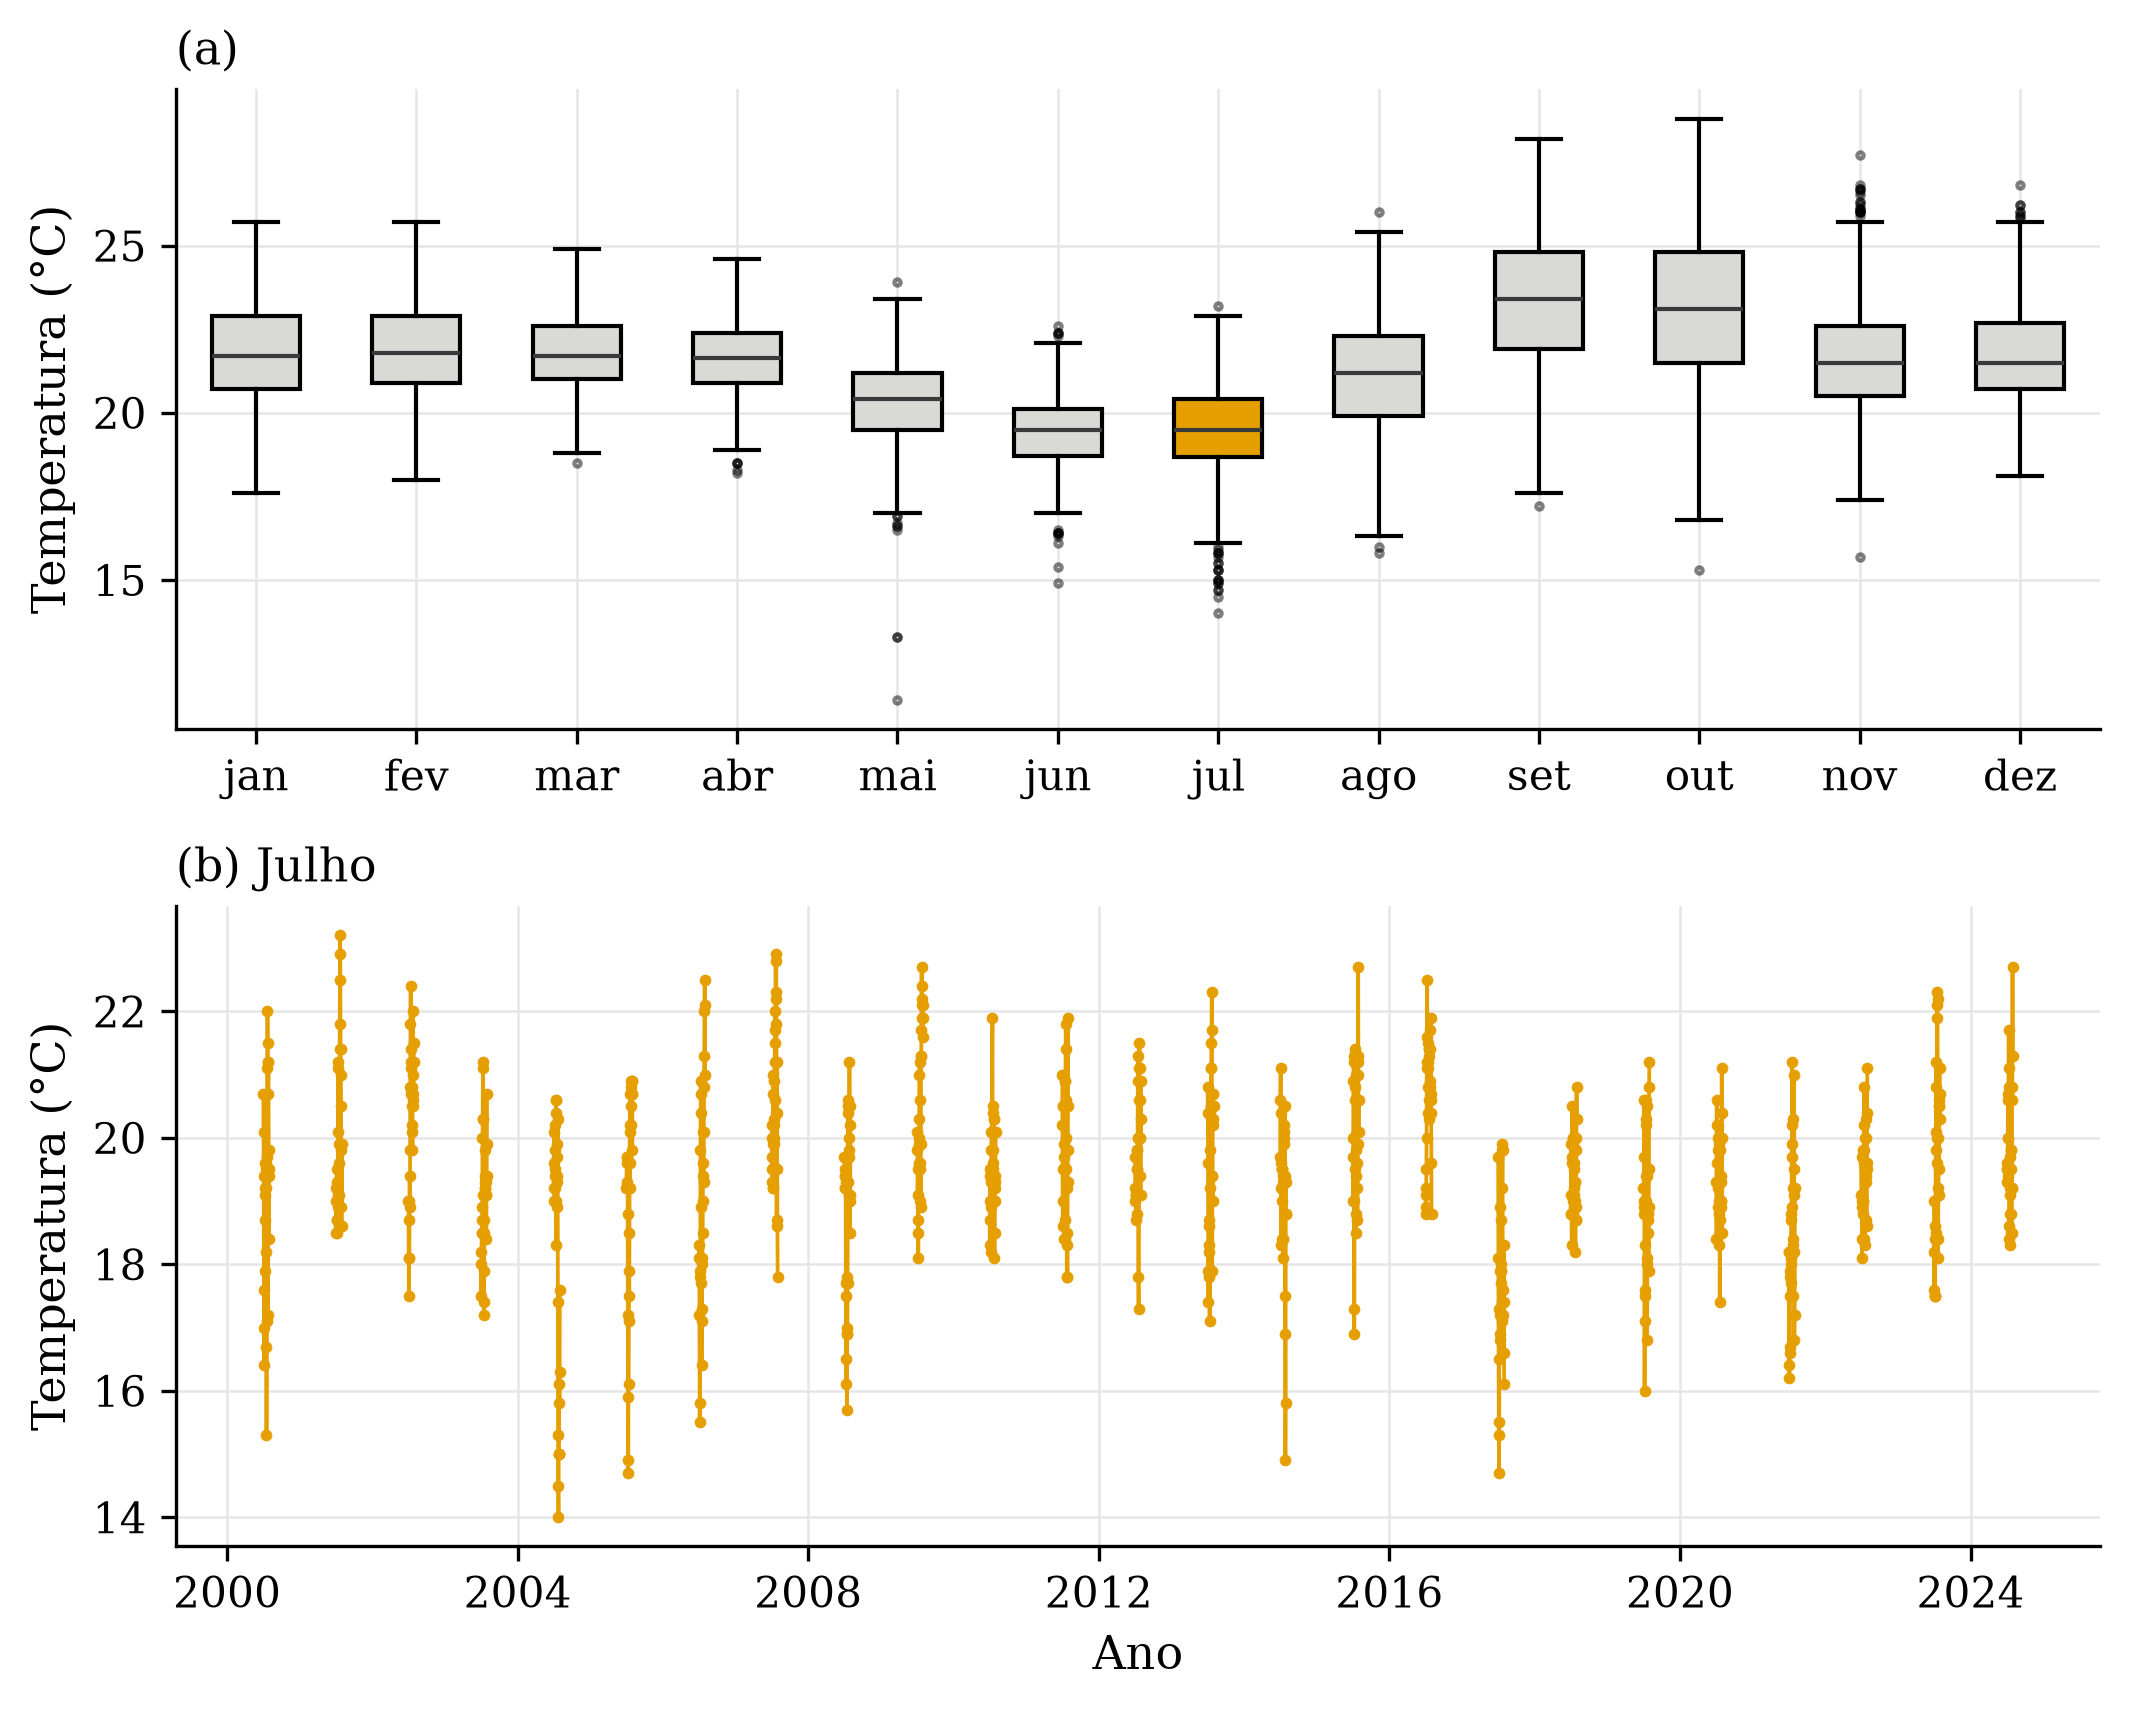
\includegraphics[width=0.85\textwidth]{figura4_temperatura_sazonalidade_pt.png}
\caption{Temperatura média diária na estação A001, com (a) a distribuição por mês, destacando julho, e (b) a série das temperaturas de julho, de 2000 a 2024.}
\label{fig:temp_sazonalidade}
\end{figure}

\subsection{Desempenho das distribuições e interpretações}

A amostra de julho (Tabela~\ref{tab:descritiva_temperatura}) apresenta temperatura média de $19,409\,^\circ\text{C}$, desvio padrão de $1,466\,^\circ\text{C}$ (com divisor $n$), assimetria moderadamente negativa ($-0,482$) e curtose de Pearson de $3,717$, isto é, um excesso de $0,717$ em relação à normal. Os quantis empíricos de 5\%, 50\% e 95\% são $16,84\,^\circ\text{C}$, $19,50\,^\circ\text{C}$ e $21,70\,^\circ\text{C}$, respectivamente.

\begin{table}[htbp]
\centering
\caption{Estatísticas descritivas da temperatura média diária de julho. Desvio padrão com divisor $n$ e curtose de Pearson (igual a $3$ para a normal).}
\label{tab:descritiva_temperatura}
\small
\begin{tabular}{lc}
\toprule
\textbf{Estatística} & \textbf{Temperatura em julho ($^\circ$C)} \\
\midrule
$n$ & 768 \\
Média & 19{,}409 \\
Mediana & 19{,}50 \\
Desvio padrão & 1{,}466 \\
Assimetria & $-0{,}482$ \\
Curtose (Pearson) & 3{,}717 \\
Mínimo; máximo & 14{,}0; 23{,}2 \\
$Q_{0{,}05}$; $Q_{0{,}50}$; $Q_{0{,}95}$ & 16{,}84; 19{,}50; 21{,}70
\unskip \\
\bottomrule
\end{tabular}
\end{table}

Aplicando o mesmo protocolo da seção~\ref{sec:vento}, comparou-se o modelo normal, com parâmetros de máxima verossimilhança $\widehat{\mu} = 19,409\,^\circ\text{C}$ e $\widehat{\sigma} = 1,466\,^\circ\text{C}$, com a GLD-FKML ajustada pelo método dos momentos com a biblioteca \texttt{pyglam}, que resultou em $\widehat{\boldsymbol\lambda} = (19,538;\, 1,0707;\, 0,0175;\, 0,1836)$.

As discrepâncias quantílicas são reportadas diretamente na unidade física ($\Delta_p$, em $^\circ$C). A Tabela~\ref{tab:desempenho_temperatura} apresenta os diagnósticos comparativos e a Figura~\ref{fig:diagnosticos_temperatura} sintetiza a sobreposição das densidades, as funções acumuladas e o gráfico Q-Q.

\begin{table}[htbp]
\centering
\caption{Desempenho dos modelos ajustados às temperaturas médias diárias de julho. As diferenças de quantis $\Delta_p$ estão em $^\circ$C.}
\label{tab:desempenho_temperatura}
\begin{tabular}{lccccc}
\toprule
\textbf{Modelo} & \textbf{Parâmetros} & \textbf{$D_n$} & \textbf{$\Delta_{0,05}$} & \textbf{$\Delta_{0,50}$} & \textbf{$\Delta_{0,95}$} \\
\midrule
Normal & 2 & 0{,}064 & +0{,}163 & -0{,}091 & +0{,}120 \\
GLD-FKML & 4 & 0{,}041 & +0{,}025 & +0{,}002 & -0{,}058
\unskip \\
\bottomrule
\end{tabular}
\end{table}

\begin{figure}[htbp]
\centering
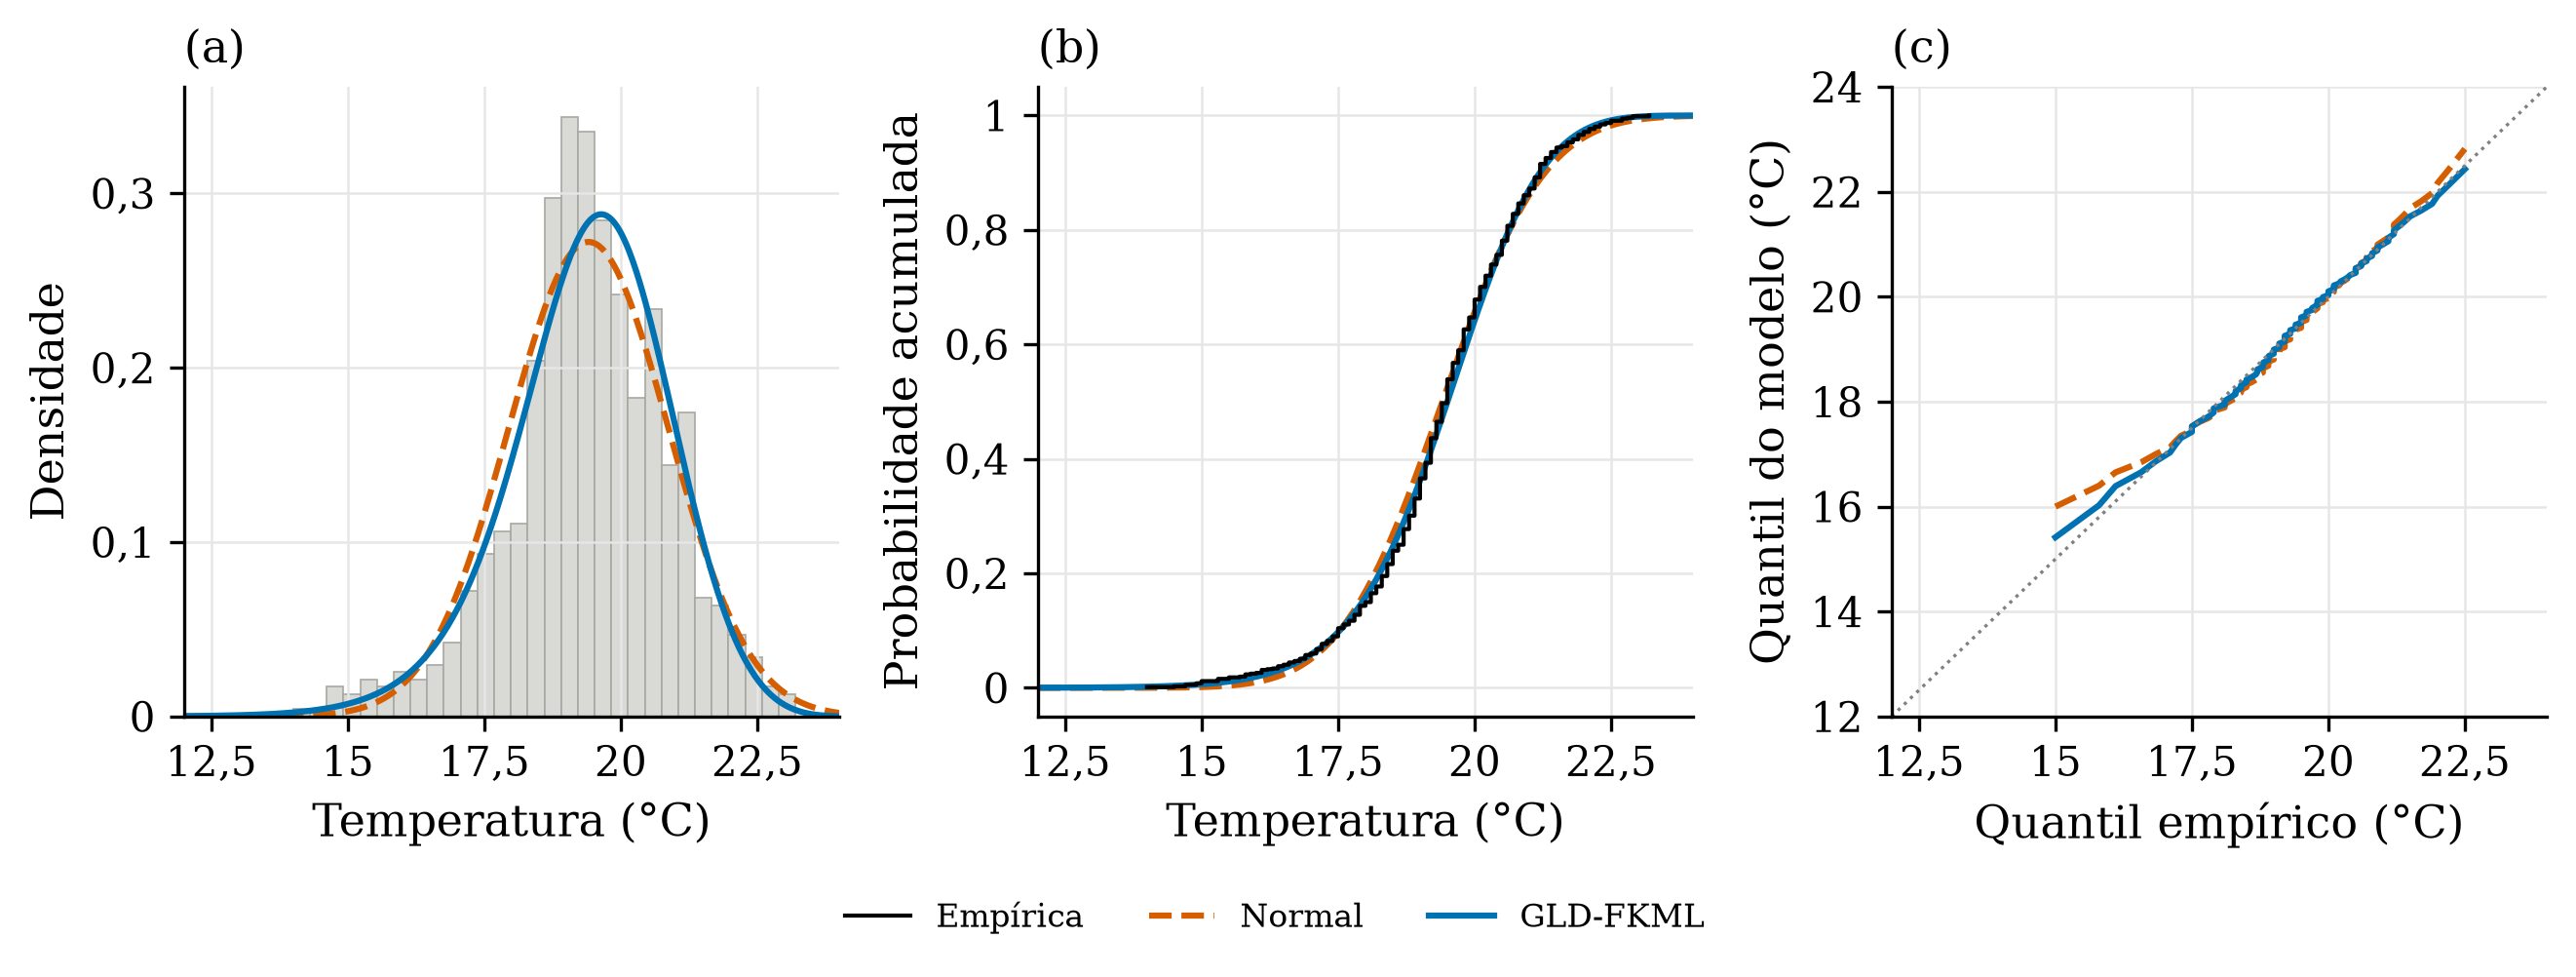
\includegraphics[width=\textwidth]{figura5_temperatura_diagnosticos_pt.png}
\caption{Diagnóstico comparativo das temperaturas de julho, com (a) densidades sobrepostas ao histograma, (b) funções distribuição acumuladas e (c) gráfico quantil-quantil, em que a linha pontilhada indica concordância perfeita. Como na Figura~\ref{fig:diagnosticos}, o gráfico Q-Q usa os percentis de 1\% a 99\%.}
\label{fig:diagnosticos_temperatura}
\end{figure}

\subsection{Interpretação didática e física}

Neste exemplo, a escolha entre a normal e a GLD-FKML recorre ao princípio da parcimônia (navalha de Ockham). A distribuição normal ajustada exibe uma distância de Kolmogorov-Smirnov pequena ($D_n = 0,064$), e os desvios quantílicos situam-se na ordem de décimos de grau Celsius ($+0,16\,^\circ\text{C}$ no quantil de 5\% e $+0,12\,^\circ\text{C}$ no de 95\%).

Para decidir se essas discrepâncias justificam um modelo mais complexo, a escala usada aqui é a incerteza amostral dos próprios quantis empíricos. A incerteza do sensor não foi incluída, porque a série não traz metadados instrumentais suficientes para estimá-la. Simulando amostras independentes de $768$ valores a partir da GLD ajustada, o desvio padrão do quantil empírico de $5\%$ é de cerca de $0{,}15\,^\circ\text{C}$, e o do quantil de $95\%$, de cerca de $0{,}09\,^\circ\text{C}$. Temperaturas de dias consecutivos, porém, são fortemente correlacionadas (coeficiente de autocorrelação de $0{,}65$), e julhos de anos diferentes podem ser sistematicamente mais frios ou mais quentes, de modo que a amostra contém menos informação independente do que sugerem os $768$ valores. Reamostrando anos inteiros por \textit{bootstrap} (Código~\ref{lst:bootstrap_anos}), o que preserva essas duas fontes de dependência, os desvios padrão dos quantis de $5\%$, $50\%$ e $95\%$ passam a $0{,}38$, $0{,}10$ e $0{,}21\,^\circ\text{C}$. As discrepâncias da normal ($+0{,}16$, $-0{,}09$ e $+0{,}12\,^\circ\text{C}$) são menores que esses desvios padrão. A comparação é descritiva, e não um teste, mas mostra que, nos três quantis examinados, a normal erra menos do que os próprios quantis variam de uma reamostra para outra. Já o valor de $D_n$ da normal, cerca do dobro do valor crítico de $5\%$ do teste de Lilliefors para observações independentes ($0{,}886/\sqrt{n} \approx 0{,}032$)~\cite{lilliefors1967}, sugere uma diferença de forma, mas a dependência entre dias torna esse valor crítico otimista, e o resultado não é conclusivo. Nesses casos, mesmo que a GLD-FKML acomode a assimetria negativa e reduza $D_n$ para $0{,}041$, com desvios quantílicos abaixo de $0{,}06\,^\circ\text{C}$, o acréscimo de dois parâmetros livres exige julgamento crítico, pois, para muitas aplicações térmicas usuais, o modelo normal de dois parâmetros oferece uma descrição simples e suficiente.

\lstinputlisting[float=htbp, caption={Incerteza dos quantis empíricos das temperaturas de julho por \textit{bootstrap} de anos inteiros.}, label=lst:bootstrap_anos]{codigo/05_bootstrap_anos.py}

O suporte da GLD ajustada reforça essa leitura. Com $\lambda_3$ e $\lambda_4$ positivos, o modelo é limitado nos dois lados, entre $-33,9\,^\circ\text{C}$ e $24,6\,^\circ\text{C}$ (calculados com os parâmetros sem arredondamento, disponíveis no material suplementar, e com os valores impressos acima obtém-se $-33,8\,^\circ\text{C}$). O limite inferior é muito sensível a $\lambda_3$, pois, com $\lambda_3 = 0,018$, por exemplo, ele passaria a cerca de $-32,3\,^\circ\text{C}$, o que já mostra que esse número não tem significado físico. O limite superior é plausível, pouco acima do máximo observado de $23,2\,^\circ\text{C}$. O inferior é fisicamente implausível para Brasília em julho, embora o modelo atribua a essa região uma probabilidade desprezível, porque $\lambda_3$ muito pequeno produz uma cauda esquerda longa e extremamente fina. Os limites do suporte, portanto, são uma consequência matemática dos parâmetros, e não devem ser lidos como limites físicos da grandeza.

Por outro lado, caso o foco resida na estimativa de eventos de frio intenso (cauda esquerda), a assimetria negativa capturada pela GLD ganha relevância. Uma explicação física plausível é a passagem ocasional de frentes frias e as incursões de ar frio de origem polar, que no inverno alcançam o Brasil Central~\cite{garreaud2000} e podem produzir dias isolados bem mais frios que a média, sem um mecanismo de mesma intensidade do lado quente. Este trabalho não associou os dias frios da amostra a eventos específicos. A explicação é, portanto, uma hipótese compatível com a assimetria observada. Os quantis estimados descrevem a variabilidade das temperaturas médias diárias no histórico observado do mês, mas não representam intervalos de confiança da média amostral, nem limites do sensor, tampouco uma previsão para um dia específico.
